\documentclass[twoside]{book}

% Packages required by doxygen
\usepackage{calc}
\usepackage{doxygen}
\usepackage{graphicx}
\usepackage[utf8]{inputenc}
\usepackage{makeidx}
\usepackage{multicol}
\usepackage{multirow}
\usepackage{textcomp}
\usepackage[table]{xcolor}

% Font selection
\usepackage[T1]{fontenc}
\usepackage{mathptmx}
\usepackage[scaled=.90]{helvet}
\usepackage{courier}
\usepackage{amssymb}
\usepackage{sectsty}
\renewcommand{\familydefault}{\sfdefault}
\allsectionsfont{%
  \fontseries{bc}\selectfont%
  \color{darkgray}%
}
\renewcommand{\DoxyLabelFont}{%
  \fontseries{bc}\selectfont%
  \color{darkgray}%
}

% Page & text layout
\usepackage{geometry}
\geometry{%
  a4paper,%
  top=2.5cm,%
  bottom=2.5cm,%
  left=2.5cm,%
  right=2.5cm%
}
\tolerance=750
\hfuzz=15pt
\hbadness=750
\setlength{\emergencystretch}{15pt}
\setlength{\parindent}{0cm}
\setlength{\parskip}{0.2cm}
\makeatletter
\renewcommand{\paragraph}{%
  \@startsection{paragraph}{4}{0ex}{-1.0ex}{1.0ex}{%
    \normalfont\normalsize\bfseries\SS@parafont%
  }%
}
\renewcommand{\subparagraph}{%
  \@startsection{subparagraph}{5}{0ex}{-1.0ex}{1.0ex}{%
    \normalfont\normalsize\bfseries\SS@subparafont%
  }%
}
\makeatother

% Headers & footers
\usepackage{fancyhdr}
\pagestyle{fancyplain}
\fancyhead[LE]{\fancyplain{}{\bfseries\thepage}}
\fancyhead[CE]{\fancyplain{}{}}
\fancyhead[RE]{\fancyplain{}{\bfseries\leftmark}}
\fancyhead[LO]{\fancyplain{}{\bfseries\rightmark}}
\fancyhead[CO]{\fancyplain{}{}}
\fancyhead[RO]{\fancyplain{}{\bfseries\thepage}}
\fancyfoot[LE]{\fancyplain{}{}}
\fancyfoot[CE]{\fancyplain{}{}}
\fancyfoot[RE]{\fancyplain{}{\bfseries\scriptsize Generated on Tue Apr 26 2016 01\-:52\-:52 for Tag\-It! by Doxygen }}
\fancyfoot[LO]{\fancyplain{}{\bfseries\scriptsize Generated on Tue Apr 26 2016 01\-:52\-:52 for Tag\-It! by Doxygen }}
\fancyfoot[CO]{\fancyplain{}{}}
\fancyfoot[RO]{\fancyplain{}{}}
\renewcommand{\footrulewidth}{0.4pt}
\renewcommand{\chaptermark}[1]{%
  \markboth{#1}{}%
}
\renewcommand{\sectionmark}[1]{%
  \markright{\thesection\ #1}%
}

% Indices & bibliography
\usepackage{natbib}
\usepackage[titles]{tocloft}
\setcounter{tocdepth}{3}
\setcounter{secnumdepth}{5}
\makeindex

% Hyperlinks (required, but should be loaded last)
\usepackage{ifpdf}
\ifpdf
  \usepackage[pdftex,pagebackref=true]{hyperref}
\else
  \usepackage[ps2pdf,pagebackref=true]{hyperref}
\fi
\hypersetup{%
  colorlinks=true,%
  linkcolor=blue,%
  citecolor=blue,%
  unicode%
}

% Custom commands
\newcommand{\clearemptydoublepage}{%
  \newpage{\pagestyle{empty}\cleardoublepage}%
}


%===== C O N T E N T S =====

\begin{document}

% Titlepage & ToC
\hypersetup{pageanchor=false}
\pagenumbering{roman}
\begin{titlepage}
\vspace*{7cm}
\begin{center}%
{\Large Tag\-It! }\\
\vspace*{1cm}
{\large Generated by Doxygen 1.8.6}\\
\vspace*{0.5cm}
{\small Tue Apr 26 2016 01:52:52}\\
\end{center}
\end{titlepage}
\clearemptydoublepage
\tableofcontents
\clearemptydoublepage
\pagenumbering{arabic}
\hypersetup{pageanchor=true}

%--- Begin generated contents ---
\chapter{Dokumentacja Tag\-It!}
\label{index}\hypertarget{index}{}\hypertarget{index_intro_sec}{}\section{Wstęp...}\label{index_intro_sec}
Tag\-It! to desktopowa aplikacja na systemy Linux, umożliwiająca wygodne, automatyczne tagowanie i nazywanie plików z muzyką, zapewniając przejrzystość w folderach. Dzięki temu można będzie łatwo odnaleźć konkretny utwór, czy też wszystkie utwory danego wykonawcy.\hypertarget{index_install_sec}{}\section{Szczegółowy opis\-:}\label{index_install_sec}
Użytkownik Tag\-It! może wskazać do przetwarzania pojedynczy plik muzyczny, po czym, zależnie od wybranych opcji nastąpi odpowiednie zmodyfikowanie jego nazwy, metadanych oraz ewentualne dodanie okładki albumu, z którego pochodzi. Po wyznaczeniu danego katalogu, aplikacja potrafi również rekurencyjnie przetworzyć znajdujące się w nim pliki, zgodnie z tym jak zostało to opisane wyżej. Ukłonem w stronę użytkownika jest opcja stworzenia i monitorowania muzycznej kolekcji z folderu, który w razie potrzeby zostanie podzielony na adekwatne podfoldery. Wówczas po dodaniu do kolekcji nowego utworu, zostanie on automatycznie nazwany i otagowany. Dzięki temu, pliki po przetworzeniu będą miały jednolity format nazw, odpowiednio zmodyfikowane dodatkowe informacje takie jak\-: gatunek muzyczny, wykonawca, nazwa zespołu, czy album, z którego pochodzą, co zapewni użytkownikowi kontrolę nad jego kolekcją audio. Oczywiście w razie potrzeby ma on również możliwość ręcznej manipulacji metadanymi z poziomu aplikacji.

Tag\-It! obsługuje najpopularniejsze formaty plików takie jak mp3, flac, wav, ogg oraz aac. Ponadto do rozpoznawania plików muzycznych, program łączy się z zewnętrzną bazą online, a więc do poprawnego działania programu wymagane jest połączenie z internetem. Sama baza danych będzie stopniowo rozbudowywana na podstawie różnorakich serwisów muzycznych, stron internetowych, czy też już aktualnie istniejących, ogólnodostępnych, internetowych baz danych przez twórców Tag\-It! oraz odpowiednie web crawlery. Program oferuje również możliwość dodania do bazy metadanych przez użytkownika, w przypadku gdy tagowanie pliku zakończyło się niepowodzeniem. 
\chapter{Namespace Index}
\section{Packages}
Here are the packages with brief descriptions (if available)\-:\begin{DoxyCompactList}
\item\contentsline{section}{\hyperlink{namespaceadd}{add} }{\pageref{namespaceadd}}{}
\item\contentsline{section}{\hyperlink{namespacecollection}{collection} }{\pageref{namespacecollection}}{}
\item\contentsline{section}{\hyperlink{namespaceconfig}{config} }{\pageref{namespaceconfig}}{}
\item\contentsline{section}{\hyperlink{namespacedatabase}{database} }{\pageref{namespacedatabase}}{}
\item\contentsline{section}{\hyperlink{namespacedbConfig}{db\-Config} }{\pageref{namespacedbConfig}}{}
\item\contentsline{section}{\hyperlink{namespaceedit}{edit} }{\pageref{namespaceedit}}{}
\item\contentsline{section}{\hyperlink{namespacefile__choose}{file\-\_\-choose} }{\pageref{namespacefile__choose}}{}
\item\contentsline{section}{\hyperlink{namespacefingerprints}{fingerprints} }{\pageref{namespacefingerprints}}{}
\item\contentsline{section}{\hyperlink{namespacerecognize}{recognize} }{\pageref{namespacerecognize}}{}
\item\contentsline{section}{\hyperlink{namespacesettings}{settings} }{\pageref{namespacesettings}}{}
\end{DoxyCompactList}

\chapter{Hierarchical Index}
\section{Class Hierarchy}
This inheritance list is sorted roughly, but not completely, alphabetically\-:\begin{DoxyCompactList}
\item Application\begin{DoxyCompactList}
\item \contentsline{section}{file\-\_\-choose.\-Application}{\pageref{classfile__choose_1_1Application}}{}
\end{DoxyCompactList}
\item Application\-Window\begin{DoxyCompactList}
\item \contentsline{section}{file\-\_\-choose.\-Main\-Window}{\pageref{classfile__choose_1_1MainWindow}}{}
\end{DoxyCompactList}
\item \contentsline{section}{edit.\-Tag\-Editor}{\pageref{classedit_1_1TagEditor}}{}
\end{DoxyCompactList}

\chapter{Class Index}
\section{Class List}
Here are the classes, structs, unions and interfaces with brief descriptions\-:\begin{DoxyCompactList}
\item\contentsline{section}{\hyperlink{classfile__choose_1_1Application}{file\-\_\-choose.\-Application} }{\pageref{classfile__choose_1_1Application}}{}
\item\contentsline{section}{\hyperlink{classfile__choose_1_1MainWindow}{file\-\_\-choose.\-Main\-Window} }{\pageref{classfile__choose_1_1MainWindow}}{}
\item\contentsline{section}{\hyperlink{classedit_1_1TagEditor}{edit.\-Tag\-Editor} }{\pageref{classedit_1_1TagEditor}}{}
\end{DoxyCompactList}

\chapter{Namespace Documentation}
\hypertarget{namespaceadd}{\section{add Namespace Reference}
\label{namespaceadd}\index{add@{add}}
}
\subsection*{Functions}
\begin{DoxyCompactItemize}
\item 
def \hyperlink{namespaceadd_a2fed564d8a86dbd10d42bd4778cb296e}{add\-Song}
\end{DoxyCompactItemize}


\subsection{Detailed Description}
\begin{DoxyVerb}    Function for adding song to database.
\end{DoxyVerb}
 

\subsection{Function Documentation}
\hypertarget{namespaceadd_a2fed564d8a86dbd10d42bd4778cb296e}{\index{add@{add}!add\-Song@{add\-Song}}
\index{add\-Song@{add\-Song}!add@{add}}
\subsubsection[{add\-Song}]{\setlength{\rightskip}{0pt plus 5cm}def add.\-add\-Song (
\begin{DoxyParamCaption}
\item[{}]{path, }
\item[{}]{tags = {\ttfamily \{\}}}
\end{DoxyParamCaption}
)}}\label{namespaceadd_a2fed564d8a86dbd10d42bd4778cb296e}
\begin{DoxyVerb}    Adds song to a database.
    Works only for mp3 files for now.
    Args:
        path: Path to the song
        tags (Optional): A dictionary of tags. If empty tags of file will by used. Title and artist are required.
    Returns:
        -1 if path does not contain a valid song.
        -2 if either artist or title is missing from tags.
        1 if successful\end{DoxyVerb}
 
\hypertarget{namespacecollection}{\section{collection Namespace Reference}
\label{namespacecollection}\index{collection@{collection}}
}
\subsection*{Functions}
\begin{DoxyCompactItemize}
\item 
def \hyperlink{namespacecollection_aefaf166aee0ea51ceafd86600e5f90bb}{move\-Up}
\item 
def \hyperlink{namespacecollection_acfea76672a57d757e0b6104507715cd2}{move\-Files}
\item 
def \hyperlink{namespacecollection_a2385617fa2cd3823939a9ad0dcfe642e}{create\-Collection}
\end{DoxyCompactItemize}


\subsection{Detailed Description}
\begin{DoxyVerb}    Functions for creating and adding files to collections.
\end{DoxyVerb}
 

\subsection{Function Documentation}
\hypertarget{namespacecollection_a2385617fa2cd3823939a9ad0dcfe642e}{\index{collection@{collection}!create\-Collection@{create\-Collection}}
\index{create\-Collection@{create\-Collection}!collection@{collection}}
\subsubsection[{create\-Collection}]{\setlength{\rightskip}{0pt plus 5cm}def collection.\-create\-Collection (
\begin{DoxyParamCaption}
\item[{}]{path}
\end{DoxyParamCaption}
)}}\label{namespacecollection_a2385617fa2cd3823939a9ad0dcfe642e}
\begin{DoxyVerb}    Creates collection from a folder.
    Creates a new folder for each artist and copies his music to this folder.
    Moves unrecognized files to "unknown" folder.
    Args:
        path: Path to folder.
    Returns:
        -1 if path is not correct.
        1 if collection was successfully created.
\end{DoxyVerb}
 \hypertarget{namespacecollection_acfea76672a57d757e0b6104507715cd2}{\index{collection@{collection}!move\-Files@{move\-Files}}
\index{move\-Files@{move\-Files}!collection@{collection}}
\subsubsection[{move\-Files}]{\setlength{\rightskip}{0pt plus 5cm}def collection.\-move\-Files (
\begin{DoxyParamCaption}
\item[{}]{path}
\end{DoxyParamCaption}
)}}\label{namespacecollection_acfea76672a57d757e0b6104507715cd2}
\begin{DoxyVerb}    Moves every file from subfolders of path to path.
    Args:
        path: Path to folder.
    Returns:
        -1 if acction was unsuccessful
        1 otherwise
\end{DoxyVerb}
 \hypertarget{namespacecollection_aefaf166aee0ea51ceafd86600e5f90bb}{\index{collection@{collection}!move\-Up@{move\-Up}}
\index{move\-Up@{move\-Up}!collection@{collection}}
\subsubsection[{move\-Up}]{\setlength{\rightskip}{0pt plus 5cm}def collection.\-move\-Up (
\begin{DoxyParamCaption}
\item[{}]{src, }
\item[{}]{dst}
\end{DoxyParamCaption}
)}}\label{namespacecollection_aefaf166aee0ea51ceafd86600e5f90bb}
\begin{DoxyVerb}    Moves all files from src to dst directory.
    Returns:
        -1 if src or dst is not a directory
\end{DoxyVerb}
 
\hypertarget{namespaceconfig}{\section{config Namespace Reference}
\label{namespaceconfig}\index{config@{config}}
}
\subsection*{Variables}
\begin{DoxyCompactItemize}
\item 
\hypertarget{namespaceconfig_adf75b22e01949f33f4a8e3a3741c61d6}{int {\bfseries D\-A\-T\-A\-\_\-\-P\-O\-I\-N\-T\-S} = 4096}\label{namespaceconfig_adf75b22e01949f33f4a8e3a3741c61d6}

\item 
\hypertarget{namespaceconfig_a6ba0dac65a9edc15d94caac768b977e0}{int {\bfseries N\-U\-M\-\_\-\-O\-V\-E\-R} = 2048}\label{namespaceconfig_a6ba0dac65a9edc15d94caac768b977e0}

\item 
\hypertarget{namespaceconfig_a87d9f28dba7fea8e6bbd5cc76704bf35}{int {\bfseries F\-R\-E\-Q} = 10000}\label{namespaceconfig_a87d9f28dba7fea8e6bbd5cc76704bf35}

\item 
\hypertarget{namespaceconfig_a8562c3d9b5fab74b94cf2df40a6c0f92}{int {\bfseries A\-M\-P\-\_\-\-M\-I\-N} = 10}\label{namespaceconfig_a8562c3d9b5fab74b94cf2df40a6c0f92}

\item 
\hypertarget{namespaceconfig_ae530affe4a1630cbdad9c1b8908b92e3}{int {\bfseries P\-E\-A\-K\-\_\-\-N\-E\-I\-G\-H\-B\-O\-R\-H\-O\-O\-D\-\_\-\-S\-I\-Z\-E} = 20}\label{namespaceconfig_ae530affe4a1630cbdad9c1b8908b92e3}

\item 
\hypertarget{namespaceconfig_a8ffaade7b10824676f14907630783969}{int {\bfseries N\-U\-M\-\_\-\-O\-F\-\_\-\-P\-E\-A\-K\-S} = 15}\label{namespaceconfig_a8ffaade7b10824676f14907630783969}

\item 
\hypertarget{namespaceconfig_a22da15753bd2f0b0b771116ea6ac6cc2}{int {\bfseries M\-A\-X\-\_\-\-T\-I\-M\-E\-\_\-\-D\-I\-F\-F} = 150}\label{namespaceconfig_a22da15753bd2f0b0b771116ea6ac6cc2}

\item 
\hypertarget{namespaceconfig_a3f3fb32c4e7458d657fa14c57f9de639}{int {\bfseries T\-H\-R\-E\-S\-H\-O\-L\-D} = 15}\label{namespaceconfig_a3f3fb32c4e7458d657fa14c57f9de639}

\end{DoxyCompactItemize}


\subsection{Detailed Description}
\begin{DoxyVerb}    Configuration file.
\end{DoxyVerb}
 
\hypertarget{namespacedatabase}{\section{database Namespace Reference}
\label{namespacedatabase}\index{database@{database}}
}
\subsection*{Functions}
\begin{DoxyCompactItemize}
\item 
def \hyperlink{namespacedatabase_a9b3549848ea8c1e8583719b7f4094988}{connect}
\item 
def \hyperlink{namespacedatabase_a082580f987765bae4f434d4f87bda68a}{get\-Tags}
\end{DoxyCompactItemize}


\subsection{Detailed Description}
\begin{DoxyVerb}    Functions for operating on database.
\end{DoxyVerb}
 

\subsection{Function Documentation}
\hypertarget{namespacedatabase_a9b3549848ea8c1e8583719b7f4094988}{\index{database@{database}!connect@{connect}}
\index{connect@{connect}!database@{database}}
\subsubsection[{connect}]{\setlength{\rightskip}{0pt plus 5cm}def database.\-connect (
\begin{DoxyParamCaption}
{}
\end{DoxyParamCaption}
)}}\label{namespacedatabase_a9b3549848ea8c1e8583719b7f4094988}
\begin{DoxyVerb}    Connects to the database using data from dbConfig.py.
    Returns:
        Handler of database connection.
\end{DoxyVerb}
 \hypertarget{namespacedatabase_a082580f987765bae4f434d4f87bda68a}{\index{database@{database}!get\-Tags@{get\-Tags}}
\index{get\-Tags@{get\-Tags}!database@{database}}
\subsubsection[{get\-Tags}]{\setlength{\rightskip}{0pt plus 5cm}def database.\-get\-Tags (
\begin{DoxyParamCaption}
\item[{}]{song\-\_\-id}
\end{DoxyParamCaption}
)}}\label{namespacedatabase_a082580f987765bae4f434d4f87bda68a}
\begin{DoxyVerb}    Gets tags of a given song.
    Args:
        song_id: id of a song in database.
    Returns:
        Dictionary containing tags of a song. If tag is missing from database its value will be represented as None.
\end{DoxyVerb}
 
\hypertarget{namespacedbConfig}{\section{db\-Config Namespace Reference}
\label{namespacedbConfig}\index{db\-Config@{db\-Config}}
}
\subsection*{Variables}
\begin{DoxyCompactItemize}
\item 
\hypertarget{namespacedbConfig_a949986ecf5f2a24833921b6beb2df3b3}{string {\bfseries D\-B\-N\-A\-M\-E} = 'music'}\label{namespacedbConfig_a949986ecf5f2a24833921b6beb2df3b3}

\item 
\hypertarget{namespacedbConfig_a10f3a3730a0b1c5f4f72671e5ae146d4}{string {\bfseries H\-O\-S\-T} = 'localhost'}\label{namespacedbConfig_a10f3a3730a0b1c5f4f72671e5ae146d4}

\item 
\hypertarget{namespacedbConfig_a16b3a8cdc5fc8cfb6eb7172825a8d52e}{string {\bfseries U\-S\-E\-R} = 'wojtek'}\label{namespacedbConfig_a16b3a8cdc5fc8cfb6eb7172825a8d52e}

\item 
\hypertarget{namespacedbConfig_a804e68b91d74ebe81656be75161f3e93}{string {\bfseries P\-A\-S\-S\-W\-D} = 'test'}\label{namespacedbConfig_a804e68b91d74ebe81656be75161f3e93}

\end{DoxyCompactItemize}


\subsection{Detailed Description}
\begin{DoxyVerb}Configuration file for database connection.
\end{DoxyVerb}
 
\hypertarget{namespaceedit}{\section{edit Namespace Reference}
\label{namespaceedit}\index{edit@{edit}}
}
\subsection*{Classes}
\begin{DoxyCompactItemize}
\item 
class \hyperlink{classedit_1_1TagEditor}{Tag\-Editor}
\end{DoxyCompactItemize}
\subsection*{Functions}
\begin{DoxyCompactItemize}
\item 
\hypertarget{namespaceedit_aa5e2ba93786984738464440f4c0caf6e}{def {\bfseries s\-None}}\label{namespaceedit_aa5e2ba93786984738464440f4c0caf6e}

\item 
\hypertarget{namespaceedit_ad34997d26392c5e40567d1740d899b54}{def {\bfseries i\-None}}\label{namespaceedit_ad34997d26392c5e40567d1740d899b54}

\item 
\hypertarget{namespaceedit_a4c503646fa860960558bb92a7934dfa3}{def {\bfseries info}}\label{namespaceedit_a4c503646fa860960558bb92a7934dfa3}

\item 
\hypertarget{namespaceedit_ae0e9b2633ec33fe8a6d74d9d009ebc9f}{def {\bfseries ups\-\_\-quest}}\label{namespaceedit_ae0e9b2633ec33fe8a6d74d9d009ebc9f}

\end{DoxyCompactItemize}


\subsection{Detailed Description}
\begin{DoxyVerb}Graphical interface for manual tag editor.
\end{DoxyVerb}
 
\hypertarget{namespacefile__choose}{\section{file\-\_\-choose Namespace Reference}
\label{namespacefile__choose}\index{file\-\_\-choose@{file\-\_\-choose}}
}
\subsection*{Classes}
\begin{DoxyCompactItemize}
\item 
class \hyperlink{classfile__choose_1_1MainWindow}{Main\-Window}
\item 
class \hyperlink{classfile__choose_1_1Application}{Application}
\end{DoxyCompactItemize}
\subsection*{Variables}
\begin{DoxyCompactItemize}
\item 
\hypertarget{namespacefile__choose_aaf648f7b09af7494312577df74bba168}{tuple {\bfseries pixbuf} = Gdk\-Pixbuf.\-Pixbuf.\-new\-\_\-from\-\_\-file('logo.\-png')}\label{namespacefile__choose_aaf648f7b09af7494312577df74bba168}

\item 
\hypertarget{namespacefile__choose_aa2d3b0b2216329fa149f6853e42a1b23}{tuple {\bfseries app} = \hyperlink{classfile__choose_1_1Application}{Application}()}\label{namespacefile__choose_aa2d3b0b2216329fa149f6853e42a1b23}

\item 
\hypertarget{namespacefile__choose_a666b7d2d723a67034fdb354b866fd30b}{tuple {\bfseries exit\-\_\-status} = app.\-run(sys.\-argv)}\label{namespacefile__choose_a666b7d2d723a67034fdb354b866fd30b}

\end{DoxyCompactItemize}


\subsection{Detailed Description}
\begin{DoxyVerb}    TagIt! GUI.
\end{DoxyVerb}
 
\hypertarget{namespacefingerprints}{\section{fingerprints Namespace Reference}
\label{namespacefingerprints}\index{fingerprints@{fingerprints}}
}
\subsection*{Functions}
\begin{DoxyCompactItemize}
\item 
def \hyperlink{namespacefingerprints_ad16038d9952756d6531d72b1a511fd2c}{generate\-Spectogram}
\item 
def \hyperlink{namespacefingerprints_ae528f9d6259d39b1d78621381a8ff75a}{get2\-D\-Peaks}
\item 
def \hyperlink{namespacefingerprints_a3559a67b49b4453274c518de642fcf63}{get\-Hashes}
\item 
def \hyperlink{namespacefingerprints_ab6735baad314e024cbe01d42ff5d5c2a}{generate\-Fingerprints}
\end{DoxyCompactItemize}


\subsection{Detailed Description}
\begin{DoxyVerb}    Functions for generating fingerprints.
    Some code based on https://github.com/worldveil/dejavu/blob/master/dejavu/fingerprint.py
\end{DoxyVerb}
 

\subsection{Function Documentation}
\hypertarget{namespacefingerprints_ab6735baad314e024cbe01d42ff5d5c2a}{\index{fingerprints@{fingerprints}!generate\-Fingerprints@{generate\-Fingerprints}}
\index{generate\-Fingerprints@{generate\-Fingerprints}!fingerprints@{fingerprints}}
\subsubsection[{generate\-Fingerprints}]{\setlength{\rightskip}{0pt plus 5cm}def fingerprints.\-generate\-Fingerprints (
\begin{DoxyParamCaption}
\item[{}]{path, }
\item[{}]{start\-Time = {\ttfamily 0}, }
\item[{}]{end\-Time = {\ttfamily 60000}}
\end{DoxyParamCaption}
)}}\label{namespacefingerprints_ab6735baad314e024cbe01d42ff5d5c2a}
\begin{DoxyVerb}    Calculates array of pairs (hash, time) for a song in a given path.
    By default samples first minute of a song.
    Args:
        path: path to song.
        startTime (Optional): time from which fingerprinting should start.
        endTime (Optional): time at which fingerprinting should end.
    Returns:
        List of pairs (hash, time).
        Empty list if path does not contain a valid music file.
\end{DoxyVerb}
 \hypertarget{namespacefingerprints_ad16038d9952756d6531d72b1a511fd2c}{\index{fingerprints@{fingerprints}!generate\-Spectogram@{generate\-Spectogram}}
\index{generate\-Spectogram@{generate\-Spectogram}!fingerprints@{fingerprints}}
\subsubsection[{generate\-Spectogram}]{\setlength{\rightskip}{0pt plus 5cm}def fingerprints.\-generate\-Spectogram (
\begin{DoxyParamCaption}
\item[{}]{song}
\end{DoxyParamCaption}
)}}\label{namespacefingerprints_ad16038d9952756d6531d72b1a511fd2c}
\begin{DoxyVerb}    Generates spectogram for a song.
    Args:
        song: AugioSegement of song of which spectogram should be created.
    Returns:
        Spectrum from matplotlib.specgram with scale changed to logarithmic.
\end{DoxyVerb}
 \hypertarget{namespacefingerprints_ae528f9d6259d39b1d78621381a8ff75a}{\index{fingerprints@{fingerprints}!get2\-D\-Peaks@{get2\-D\-Peaks}}
\index{get2\-D\-Peaks@{get2\-D\-Peaks}!fingerprints@{fingerprints}}
\subsubsection[{get2\-D\-Peaks}]{\setlength{\rightskip}{0pt plus 5cm}def fingerprints.\-get2\-D\-Peaks (
\begin{DoxyParamCaption}
\item[{}]{arr2\-D}
\end{DoxyParamCaption}
)}}\label{namespacefingerprints_ae528f9d6259d39b1d78621381a8ff75a}
\begin{DoxyVerb}    Generates peaks of a spectogram.
    Args:
        arr2D: spectogram.
    Returns:
        List of pairs (time, frequency) of peaks.
\end{DoxyVerb}
 \hypertarget{namespacefingerprints_a3559a67b49b4453274c518de642fcf63}{\index{fingerprints@{fingerprints}!get\-Hashes@{get\-Hashes}}
\index{get\-Hashes@{get\-Hashes}!fingerprints@{fingerprints}}
\subsubsection[{get\-Hashes}]{\setlength{\rightskip}{0pt plus 5cm}def fingerprints.\-get\-Hashes (
\begin{DoxyParamCaption}
\item[{}]{peaks}
\end{DoxyParamCaption}
)}}\label{namespacefingerprints_a3559a67b49b4453274c518de642fcf63}
\begin{DoxyVerb}    Generates hashes of peaks.
    Args:
        peaks: list of pairs (time, frequenct) of peaks.
    Returns:
        List of pairs (hash, time).
\end{DoxyVerb}
 
\hypertarget{namespacerecognize}{\section{recognize Namespace Reference}
\label{namespacerecognize}\index{recognize@{recognize}}
}
\subsection*{Functions}
\begin{DoxyCompactItemize}
\item 
def \hyperlink{namespacerecognize_a61509c867407ec3f7533ed5aa3a6a3d4}{fingerprint\-Recognize}
\item 
def \hyperlink{namespacerecognize_a1aaeb8ac53f078425fc2fb10f222b92c}{recognize}
\end{DoxyCompactItemize}


\subsection{Detailed Description}
\begin{DoxyVerb}Functions for music files recognition.
\end{DoxyVerb}
 

\subsection{Function Documentation}
\hypertarget{namespacerecognize_a61509c867407ec3f7533ed5aa3a6a3d4}{\index{recognize@{recognize}!fingerprint\-Recognize@{fingerprint\-Recognize}}
\index{fingerprint\-Recognize@{fingerprint\-Recognize}!recognize@{recognize}}
\subsubsection[{fingerprint\-Recognize}]{\setlength{\rightskip}{0pt plus 5cm}def recognize.\-fingerprint\-Recognize (
\begin{DoxyParamCaption}
\item[{}]{path}
\end{DoxyParamCaption}
)}}\label{namespacerecognize_a61509c867407ec3f7533ed5aa3a6a3d4}
\begin{DoxyVerb}    Recognizes song using fingerprinting.
    Args:
        path: path to the song.
    Returns:
        id of a song in databse if song was found.
        -1 if song was not recognized or path does not contain a valid audio file.
\end{DoxyVerb}
 \hypertarget{namespacerecognize_a1aaeb8ac53f078425fc2fb10f222b92c}{\index{recognize@{recognize}!recognize@{recognize}}
\index{recognize@{recognize}!recognize@{recognize}}
\subsubsection[{recognize}]{\setlength{\rightskip}{0pt plus 5cm}def recognize.\-recognize (
\begin{DoxyParamCaption}
\item[{}]{path}
\end{DoxyParamCaption}
)}}\label{namespacerecognize_a1aaeb8ac53f078425fc2fb10f222b92c}
\begin{DoxyVerb}    Recognizes song from path.
    Args:
        path: path to the song.
    Returns:
        id of a song in databse if song was found.
        -1 if song was not recognized or path does not contain a valid audio file.
\end{DoxyVerb}
 
\hypertarget{namespacesettings}{\section{settings Namespace Reference}
\label{namespacesettings}\index{settings@{settings}}
}
\subsection*{Functions}
\begin{DoxyCompactItemize}
\item 
\hypertarget{namespacesettings_aae2a6ccd78a88e4c9f83031a65d31e2f}{def {\bfseries rename}}\label{namespacesettings_aae2a6ccd78a88e4c9f83031a65d31e2f}

\item 
\hypertarget{namespacesettings_a1ffda0346e434f50151fbef912722b42}{def {\bfseries save\-\_\-format\-\_\-callback}}\label{namespacesettings_a1ffda0346e434f50151fbef912722b42}

\item 
def \hyperlink{namespacesettings_a98e38e7530a3d3ec2db65938e8e53614}{change\-\_\-format}
\end{DoxyCompactItemize}
\subsection*{Variables}
\begin{DoxyCompactItemize}
\item 
\hypertarget{namespacesettings_aa8fa4ed3d1f77dedfca48dfb30fc87f5}{int {\bfseries \-\_\-name\-\_\-option} = 1}\label{namespacesettings_aa8fa4ed3d1f77dedfca48dfb30fc87f5}

\end{DoxyCompactItemize}


\subsection{Detailed Description}
\begin{DoxyVerb}Graphical interface for settings.
\end{DoxyVerb}
 

\subsection{Function Documentation}
\hypertarget{namespacesettings_a98e38e7530a3d3ec2db65938e8e53614}{\index{settings@{settings}!change\-\_\-format@{change\-\_\-format}}
\index{change\-\_\-format@{change\-\_\-format}!settings@{settings}}
\subsubsection[{change\-\_\-format}]{\setlength{\rightskip}{0pt plus 5cm}def settings.\-change\-\_\-format (
\begin{DoxyParamCaption}
\item[{}]{action, }
\item[{}]{parameter}
\end{DoxyParamCaption}
)}}\label{namespacesettings_a98e38e7530a3d3ec2db65938e8e53614}
\begin{DoxyVerb}    Shows format costumizer's window.
\end{DoxyVerb}
 
\chapter{Class Documentation}
\hypertarget{classfile__choose_1_1Application}{\section{file\-\_\-choose.\-Application Class Reference}
\label{classfile__choose_1_1Application}\index{file\-\_\-choose.\-Application@{file\-\_\-choose.\-Application}}
}
Inheritance diagram for file\-\_\-choose.\-Application\-:\begin{figure}[H]
\begin{center}
\leavevmode
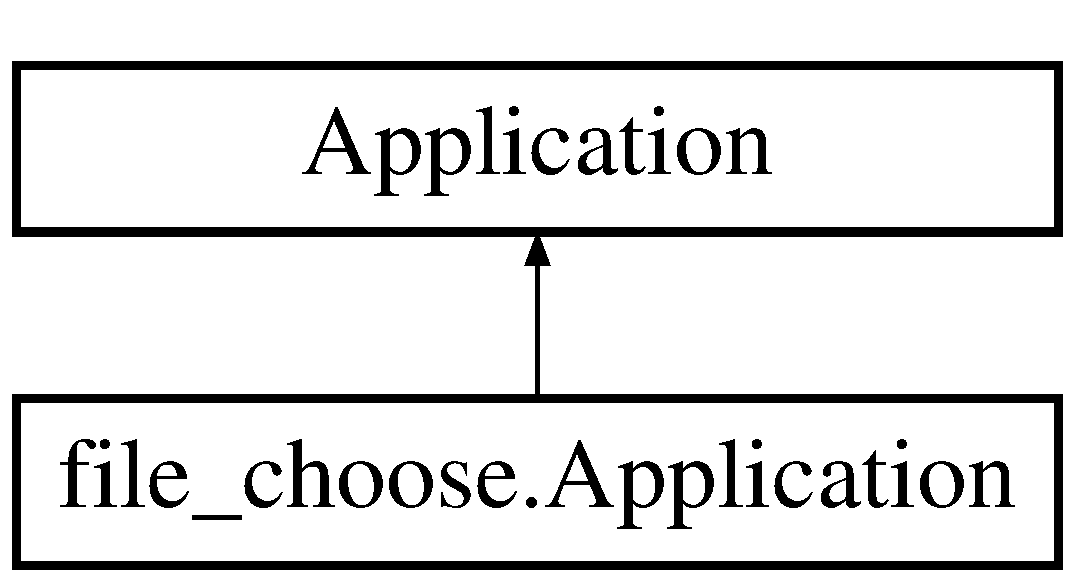
\includegraphics[height=2.000000cm]{classfile__choose_1_1Application}
\end{center}
\end{figure}
\subsection*{Public Member Functions}
\begin{DoxyCompactItemize}
\item 
def \hyperlink{classfile__choose_1_1Application_adaa9d326d0956fc7c263adab5180fa9e}{\-\_\-\-\_\-init\-\_\-\-\_\-}
\item 
\hypertarget{classfile__choose_1_1Application_a84117f4c23ed6c8d28b21030a00222c4}{def {\bfseries do\-\_\-activate}}\label{classfile__choose_1_1Application_a84117f4c23ed6c8d28b21030a00222c4}

\item 
\hypertarget{classfile__choose_1_1Application_a61b7c24fd214da3ed652211104036746}{def {\bfseries do\-\_\-startup}}\label{classfile__choose_1_1Application_a61b7c24fd214da3ed652211104036746}

\item 
def \hyperlink{classfile__choose_1_1Application_a9c93905ffb03c7ee41cf77681ff57883}{quit\-\_\-callback}
\end{DoxyCompactItemize}


\subsection{Constructor \& Destructor Documentation}
\hypertarget{classfile__choose_1_1Application_adaa9d326d0956fc7c263adab5180fa9e}{\index{file\-\_\-choose\-::\-Application@{file\-\_\-choose\-::\-Application}!\-\_\-\-\_\-init\-\_\-\-\_\-@{\-\_\-\-\_\-init\-\_\-\-\_\-}}
\index{\-\_\-\-\_\-init\-\_\-\-\_\-@{\-\_\-\-\_\-init\-\_\-\-\_\-}!file_choose::Application@{file\-\_\-choose\-::\-Application}}
\subsubsection[{\-\_\-\-\_\-init\-\_\-\-\_\-}]{\setlength{\rightskip}{0pt plus 5cm}def file\-\_\-choose.\-Application.\-\_\-\-\_\-init\-\_\-\-\_\- (
\begin{DoxyParamCaption}
\item[{}]{self}
\end{DoxyParamCaption}
)}}\label{classfile__choose_1_1Application_adaa9d326d0956fc7c263adab5180fa9e}
\begin{DoxyVerb}    Application constructor.
\end{DoxyVerb}
 

\subsection{Member Function Documentation}
\hypertarget{classfile__choose_1_1Application_a9c93905ffb03c7ee41cf77681ff57883}{\index{file\-\_\-choose\-::\-Application@{file\-\_\-choose\-::\-Application}!quit\-\_\-callback@{quit\-\_\-callback}}
\index{quit\-\_\-callback@{quit\-\_\-callback}!file_choose::Application@{file\-\_\-choose\-::\-Application}}
\subsubsection[{quit\-\_\-callback}]{\setlength{\rightskip}{0pt plus 5cm}def file\-\_\-choose.\-Application.\-quit\-\_\-callback (
\begin{DoxyParamCaption}
\item[{}]{self, }
\item[{}]{action, }
\item[{}]{parameter}
\end{DoxyParamCaption}
)}}\label{classfile__choose_1_1Application_a9c93905ffb03c7ee41cf77681ff57883}
\begin{DoxyVerb}    Callback function for quit.
\end{DoxyVerb}
 

The documentation for this class was generated from the following file\-:\begin{DoxyCompactItemize}
\item 
file\-\_\-choose.\-py\end{DoxyCompactItemize}

\hypertarget{classfile__choose_1_1MainWindow}{\section{file\-\_\-choose.\-Main\-Window Class Reference}
\label{classfile__choose_1_1MainWindow}\index{file\-\_\-choose.\-Main\-Window@{file\-\_\-choose.\-Main\-Window}}
}
Inheritance diagram for file\-\_\-choose.\-Main\-Window\-:\begin{figure}[H]
\begin{center}
\leavevmode
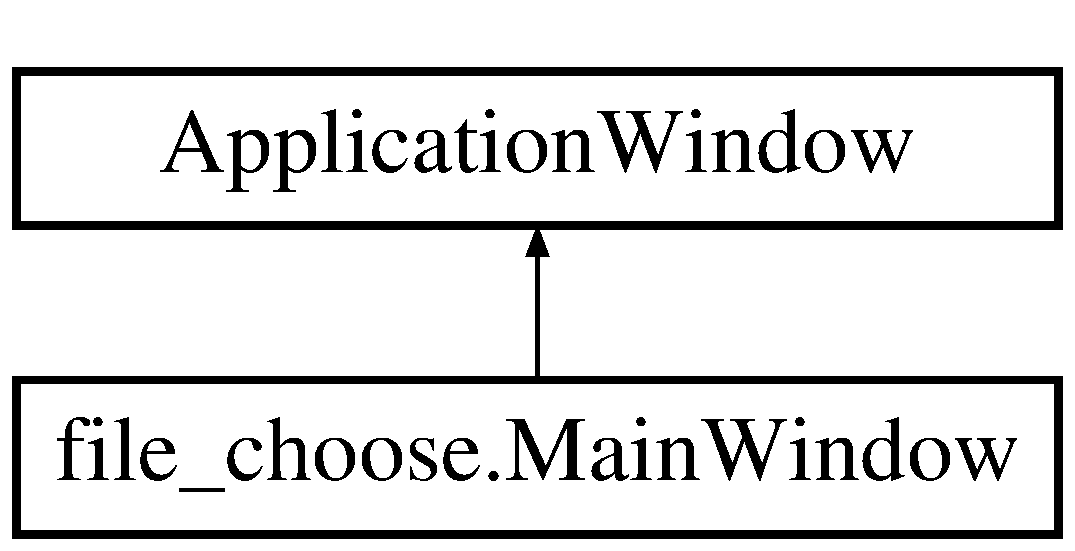
\includegraphics[height=2.000000cm]{classfile__choose_1_1MainWindow}
\end{center}
\end{figure}
\subsection*{Public Member Functions}
\begin{DoxyCompactItemize}
\item 
def \hyperlink{classfile__choose_1_1MainWindow_a0d10e7e4a44d9780107288dc2dd9220b}{\-\_\-\-\_\-init\-\_\-\-\_\-}
\item 
def \hyperlink{classfile__choose_1_1MainWindow_ad49cfa9f160158a7e3a83cd24b01a31e}{col\-\_\-open\-\_\-callback}
\item 
def \hyperlink{classfile__choose_1_1MainWindow_a011d718bd622d069252e78dc5f0938f7}{col\-\_\-open\-\_\-response\-\_\-cb}
\item 
def \hyperlink{classfile__choose_1_1MainWindow_aeecbe5035b03dd6a49948ea656c6659d}{tag\-Edit\-\_\-callback}
\item 
def \hyperlink{classfile__choose_1_1MainWindow_a0f30fd7eb17c3927de393ccabcabb7e0}{about\-\_\-callback}
\item 
def \hyperlink{classfile__choose_1_1MainWindow_a370aa9406738d9718cf447557d4e4890}{on\-\_\-close}
\item 
def \hyperlink{classfile__choose_1_1MainWindow_ab88fee4368005a828bd4dc8f5630a0ef}{settings\-\_\-callback}
\item 
def \hyperlink{classfile__choose_1_1MainWindow_aac9eb94882ec19e2163aee20e36a1e60}{open\-\_\-callback}
\item 
def \hyperlink{classfile__choose_1_1MainWindow_a31529647c093eee7092cd6a747d89115}{open\-\_\-response\-\_\-cb}
\item 
def \hyperlink{classfile__choose_1_1MainWindow_a5d333707ccd3ce7f0a53ddb40879a968}{dir\-\_\-open\-\_\-callback}
\item 
def \hyperlink{classfile__choose_1_1MainWindow_a1605c35552ab074ae261c58142b18887}{dir\-\_\-open\-\_\-response\-\_\-cb}
\end{DoxyCompactItemize}


\subsection{Constructor \& Destructor Documentation}
\hypertarget{classfile__choose_1_1MainWindow_a0d10e7e4a44d9780107288dc2dd9220b}{\index{file\-\_\-choose\-::\-Main\-Window@{file\-\_\-choose\-::\-Main\-Window}!\-\_\-\-\_\-init\-\_\-\-\_\-@{\-\_\-\-\_\-init\-\_\-\-\_\-}}
\index{\-\_\-\-\_\-init\-\_\-\-\_\-@{\-\_\-\-\_\-init\-\_\-\-\_\-}!file_choose::MainWindow@{file\-\_\-choose\-::\-Main\-Window}}
\subsubsection[{\-\_\-\-\_\-init\-\_\-\-\_\-}]{\setlength{\rightskip}{0pt plus 5cm}def file\-\_\-choose.\-Main\-Window.\-\_\-\-\_\-init\-\_\-\-\_\- (
\begin{DoxyParamCaption}
\item[{}]{self, }
\item[{}]{app}
\end{DoxyParamCaption}
)}}\label{classfile__choose_1_1MainWindow_a0d10e7e4a44d9780107288dc2dd9220b}
\begin{DoxyVerb}    MainWindow constructor.
\end{DoxyVerb}
 

\subsection{Member Function Documentation}
\hypertarget{classfile__choose_1_1MainWindow_a0f30fd7eb17c3927de393ccabcabb7e0}{\index{file\-\_\-choose\-::\-Main\-Window@{file\-\_\-choose\-::\-Main\-Window}!about\-\_\-callback@{about\-\_\-callback}}
\index{about\-\_\-callback@{about\-\_\-callback}!file_choose::MainWindow@{file\-\_\-choose\-::\-Main\-Window}}
\subsubsection[{about\-\_\-callback}]{\setlength{\rightskip}{0pt plus 5cm}def file\-\_\-choose.\-Main\-Window.\-about\-\_\-callback (
\begin{DoxyParamCaption}
\item[{}]{self, }
\item[{}]{action, }
\item[{}]{parameter}
\end{DoxyParamCaption}
)}}\label{classfile__choose_1_1MainWindow_a0f30fd7eb17c3927de393ccabcabb7e0}
\begin{DoxyVerb}    Callback function for about.
\end{DoxyVerb}
 \hypertarget{classfile__choose_1_1MainWindow_ad49cfa9f160158a7e3a83cd24b01a31e}{\index{file\-\_\-choose\-::\-Main\-Window@{file\-\_\-choose\-::\-Main\-Window}!col\-\_\-open\-\_\-callback@{col\-\_\-open\-\_\-callback}}
\index{col\-\_\-open\-\_\-callback@{col\-\_\-open\-\_\-callback}!file_choose::MainWindow@{file\-\_\-choose\-::\-Main\-Window}}
\subsubsection[{col\-\_\-open\-\_\-callback}]{\setlength{\rightskip}{0pt plus 5cm}def file\-\_\-choose.\-Main\-Window.\-col\-\_\-open\-\_\-callback (
\begin{DoxyParamCaption}
\item[{}]{self, }
\item[{}]{action, }
\item[{}]{parameter}
\end{DoxyParamCaption}
)}}\label{classfile__choose_1_1MainWindow_ad49cfa9f160158a7e3a83cd24b01a31e}
\begin{DoxyVerb}    Callback for creating collection.
\end{DoxyVerb}
 \hypertarget{classfile__choose_1_1MainWindow_a011d718bd622d069252e78dc5f0938f7}{\index{file\-\_\-choose\-::\-Main\-Window@{file\-\_\-choose\-::\-Main\-Window}!col\-\_\-open\-\_\-response\-\_\-cb@{col\-\_\-open\-\_\-response\-\_\-cb}}
\index{col\-\_\-open\-\_\-response\-\_\-cb@{col\-\_\-open\-\_\-response\-\_\-cb}!file_choose::MainWindow@{file\-\_\-choose\-::\-Main\-Window}}
\subsubsection[{col\-\_\-open\-\_\-response\-\_\-cb}]{\setlength{\rightskip}{0pt plus 5cm}def file\-\_\-choose.\-Main\-Window.\-col\-\_\-open\-\_\-response\-\_\-cb (
\begin{DoxyParamCaption}
\item[{}]{self, }
\item[{}]{dialog, }
\item[{}]{response\-\_\-id}
\end{DoxyParamCaption}
)}}\label{classfile__choose_1_1MainWindow_a011d718bd622d069252e78dc5f0938f7}
\begin{DoxyVerb}    Callback function for the dialog col_open_dialog.
\end{DoxyVerb}
 \hypertarget{classfile__choose_1_1MainWindow_a5d333707ccd3ce7f0a53ddb40879a968}{\index{file\-\_\-choose\-::\-Main\-Window@{file\-\_\-choose\-::\-Main\-Window}!dir\-\_\-open\-\_\-callback@{dir\-\_\-open\-\_\-callback}}
\index{dir\-\_\-open\-\_\-callback@{dir\-\_\-open\-\_\-callback}!file_choose::MainWindow@{file\-\_\-choose\-::\-Main\-Window}}
\subsubsection[{dir\-\_\-open\-\_\-callback}]{\setlength{\rightskip}{0pt plus 5cm}def file\-\_\-choose.\-Main\-Window.\-dir\-\_\-open\-\_\-callback (
\begin{DoxyParamCaption}
\item[{}]{self, }
\item[{}]{action, }
\item[{}]{parameter}
\end{DoxyParamCaption}
)}}\label{classfile__choose_1_1MainWindow_a5d333707ccd3ce7f0a53ddb40879a968}
\begin{DoxyVerb}    Callback for open a directory.
\end{DoxyVerb}
 \hypertarget{classfile__choose_1_1MainWindow_a1605c35552ab074ae261c58142b18887}{\index{file\-\_\-choose\-::\-Main\-Window@{file\-\_\-choose\-::\-Main\-Window}!dir\-\_\-open\-\_\-response\-\_\-cb@{dir\-\_\-open\-\_\-response\-\_\-cb}}
\index{dir\-\_\-open\-\_\-response\-\_\-cb@{dir\-\_\-open\-\_\-response\-\_\-cb}!file_choose::MainWindow@{file\-\_\-choose\-::\-Main\-Window}}
\subsubsection[{dir\-\_\-open\-\_\-response\-\_\-cb}]{\setlength{\rightskip}{0pt plus 5cm}def file\-\_\-choose.\-Main\-Window.\-dir\-\_\-open\-\_\-response\-\_\-cb (
\begin{DoxyParamCaption}
\item[{}]{self, }
\item[{}]{dialog, }
\item[{}]{response\-\_\-id}
\end{DoxyParamCaption}
)}}\label{classfile__choose_1_1MainWindow_a1605c35552ab074ae261c58142b18887}
\begin{DoxyVerb}    Callback function for the dialog dir_open_dialog.
\end{DoxyVerb}
 \hypertarget{classfile__choose_1_1MainWindow_a370aa9406738d9718cf447557d4e4890}{\index{file\-\_\-choose\-::\-Main\-Window@{file\-\_\-choose\-::\-Main\-Window}!on\-\_\-close@{on\-\_\-close}}
\index{on\-\_\-close@{on\-\_\-close}!file_choose::MainWindow@{file\-\_\-choose\-::\-Main\-Window}}
\subsubsection[{on\-\_\-close}]{\setlength{\rightskip}{0pt plus 5cm}def file\-\_\-choose.\-Main\-Window.\-on\-\_\-close (
\begin{DoxyParamCaption}
\item[{}]{self, }
\item[{}]{action, }
\item[{}]{parameter}
\end{DoxyParamCaption}
)}}\label{classfile__choose_1_1MainWindow_a370aa9406738d9718cf447557d4e4890}
\begin{DoxyVerb}    A callback function to destroy the about dialog.
\end{DoxyVerb}
 \hypertarget{classfile__choose_1_1MainWindow_aac9eb94882ec19e2163aee20e36a1e60}{\index{file\-\_\-choose\-::\-Main\-Window@{file\-\_\-choose\-::\-Main\-Window}!open\-\_\-callback@{open\-\_\-callback}}
\index{open\-\_\-callback@{open\-\_\-callback}!file_choose::MainWindow@{file\-\_\-choose\-::\-Main\-Window}}
\subsubsection[{open\-\_\-callback}]{\setlength{\rightskip}{0pt plus 5cm}def file\-\_\-choose.\-Main\-Window.\-open\-\_\-callback (
\begin{DoxyParamCaption}
\item[{}]{self, }
\item[{}]{action, }
\item[{}]{parameter}
\end{DoxyParamCaption}
)}}\label{classfile__choose_1_1MainWindow_aac9eb94882ec19e2163aee20e36a1e60}
\begin{DoxyVerb}    Callback for open.
\end{DoxyVerb}
 \hypertarget{classfile__choose_1_1MainWindow_a31529647c093eee7092cd6a747d89115}{\index{file\-\_\-choose\-::\-Main\-Window@{file\-\_\-choose\-::\-Main\-Window}!open\-\_\-response\-\_\-cb@{open\-\_\-response\-\_\-cb}}
\index{open\-\_\-response\-\_\-cb@{open\-\_\-response\-\_\-cb}!file_choose::MainWindow@{file\-\_\-choose\-::\-Main\-Window}}
\subsubsection[{open\-\_\-response\-\_\-cb}]{\setlength{\rightskip}{0pt plus 5cm}def file\-\_\-choose.\-Main\-Window.\-open\-\_\-response\-\_\-cb (
\begin{DoxyParamCaption}
\item[{}]{self, }
\item[{}]{dialog, }
\item[{}]{response\-\_\-id}
\end{DoxyParamCaption}
)}}\label{classfile__choose_1_1MainWindow_a31529647c093eee7092cd6a747d89115}
\begin{DoxyVerb}    Callback function for the dialog open_dialog.
\end{DoxyVerb}
 \hypertarget{classfile__choose_1_1MainWindow_ab88fee4368005a828bd4dc8f5630a0ef}{\index{file\-\_\-choose\-::\-Main\-Window@{file\-\_\-choose\-::\-Main\-Window}!settings\-\_\-callback@{settings\-\_\-callback}}
\index{settings\-\_\-callback@{settings\-\_\-callback}!file_choose::MainWindow@{file\-\_\-choose\-::\-Main\-Window}}
\subsubsection[{settings\-\_\-callback}]{\setlength{\rightskip}{0pt plus 5cm}def file\-\_\-choose.\-Main\-Window.\-settings\-\_\-callback (
\begin{DoxyParamCaption}
\item[{}]{self, }
\item[{}]{action, }
\item[{}]{parameter}
\end{DoxyParamCaption}
)}}\label{classfile__choose_1_1MainWindow_ab88fee4368005a828bd4dc8f5630a0ef}
\begin{DoxyVerb}    Callback for settings.
\end{DoxyVerb}
 \hypertarget{classfile__choose_1_1MainWindow_aeecbe5035b03dd6a49948ea656c6659d}{\index{file\-\_\-choose\-::\-Main\-Window@{file\-\_\-choose\-::\-Main\-Window}!tag\-Edit\-\_\-callback@{tag\-Edit\-\_\-callback}}
\index{tag\-Edit\-\_\-callback@{tag\-Edit\-\_\-callback}!file_choose::MainWindow@{file\-\_\-choose\-::\-Main\-Window}}
\subsubsection[{tag\-Edit\-\_\-callback}]{\setlength{\rightskip}{0pt plus 5cm}def file\-\_\-choose.\-Main\-Window.\-tag\-Edit\-\_\-callback (
\begin{DoxyParamCaption}
\item[{}]{self, }
\item[{}]{action, }
\item[{}]{parameter}
\end{DoxyParamCaption}
)}}\label{classfile__choose_1_1MainWindow_aeecbe5035b03dd6a49948ea656c6659d}
\begin{DoxyVerb}    Callback function for tagEditor.
\end{DoxyVerb}
 

The documentation for this class was generated from the following file\-:\begin{DoxyCompactItemize}
\item 
file\-\_\-choose.\-py\end{DoxyCompactItemize}

\hypertarget{classedit_1_1TagEditor}{\section{edit.\-Tag\-Editor Class Reference}
\label{classedit_1_1TagEditor}\index{edit.\-Tag\-Editor@{edit.\-Tag\-Editor}}
}
\subsection*{Public Member Functions}
\begin{DoxyCompactItemize}
\item 
\hypertarget{classedit_1_1TagEditor_a32b9ed3edf034376e542a831212ed2bc}{def {\bfseries \-\_\-\-\_\-init\-\_\-\-\_\-}}\label{classedit_1_1TagEditor_a32b9ed3edf034376e542a831212ed2bc}

\item 
\hypertarget{classedit_1_1TagEditor_a514af08ad751f6368971cb94121c0d48}{def {\bfseries error\-Opening}}\label{classedit_1_1TagEditor_a514af08ad751f6368971cb94121c0d48}

\item 
\hypertarget{classedit_1_1TagEditor_a953ca2da4185dfaeedda31ffd5d9dd2d}{def {\bfseries cancel\-\_\-callback}}\label{classedit_1_1TagEditor_a953ca2da4185dfaeedda31ffd5d9dd2d}

\item 
\hypertarget{classedit_1_1TagEditor_a79e286c1c2d95c1c43b47526bd7b2682}{def {\bfseries save\-\_\-callback}}\label{classedit_1_1TagEditor_a79e286c1c2d95c1c43b47526bd7b2682}

\item 
def \hyperlink{classedit_1_1TagEditor_ab076fe635a4fcbed39d688322a5013b0}{tag\-Editor}
\end{DoxyCompactItemize}
\subsection*{Public Attributes}
\begin{DoxyCompactItemize}
\item 
\hypertarget{classedit_1_1TagEditor_adb26284bfa6ad0f42b164666f33ea1be}{{\bfseries filename}}\label{classedit_1_1TagEditor_adb26284bfa6ad0f42b164666f33ea1be}

\end{DoxyCompactItemize}
\subsection*{Static Public Attributes}
\begin{DoxyCompactItemize}
\item 
\hypertarget{classedit_1_1TagEditor_afa98963cc6e756dbcd68b40f5b9abf83}{tuple {\bfseries builder} = Gtk.\-Builder()}\label{classedit_1_1TagEditor_afa98963cc6e756dbcd68b40f5b9abf83}

\end{DoxyCompactItemize}


\subsection{Detailed Description}
\begin{DoxyVerb}    Every instance of this class creates window that enables
    user to manually change tags for given file. Requires
    filepath passed to constructor.
\end{DoxyVerb}
 

\subsection{Member Function Documentation}
\hypertarget{classedit_1_1TagEditor_ab076fe635a4fcbed39d688322a5013b0}{\index{edit\-::\-Tag\-Editor@{edit\-::\-Tag\-Editor}!tag\-Editor@{tag\-Editor}}
\index{tag\-Editor@{tag\-Editor}!edit::TagEditor@{edit\-::\-Tag\-Editor}}
\subsubsection[{tag\-Editor}]{\setlength{\rightskip}{0pt plus 5cm}def edit.\-Tag\-Editor.\-tag\-Editor (
\begin{DoxyParamCaption}
\item[{}]{self}
\end{DoxyParamCaption}
)}}\label{classedit_1_1TagEditor_ab076fe635a4fcbed39d688322a5013b0}
\begin{DoxyVerb}  Shows editor's window.
\end{DoxyVerb}
 

The documentation for this class was generated from the following file\-:\begin{DoxyCompactItemize}
\item 
edit.\-py\end{DoxyCompactItemize}

%--- End generated contents ---

% Index
\newpage
\phantomsection
\addcontentsline{toc}{chapter}{Index}
\printindex

\end{document}
